\documentclass[11pt,leqno]{beamer}
\usepackage{makecell}
\usepackage{ifxetex}
\usepackage{xcolor}
\ifxetex

  \usepackage[T1]{fontenc}
  \usepackage[no-math]{fontspec}

  \usefonttheme{serif}
  \setmainfont{Times NR MT Std}
H
  \usepackage[cal=euler, calscaled=1.0,
	      scr=boondox, scrscaled=1.0]{mathalfa}

  \let\hbar\relax
  \usepackage[noamssymbols,mtpcal,mtphrb,mtpfrak,
  	      subscriptcorrection,zswash]{mtpro2}
\else
  %\usepackage{lmodern}
  %\usepackage{mathrsfs}
  \usefonttheme{professionalfonts}
  \usepackage{stix}
  \newcommand{\mbf}{\mathbf} % to match mt2pro
\fi

\usetheme{metropolis}
\usepackage{appendixnumberbeamer}

%\usepackage{booktabs}
%\usepackage[scale=2]{ccicons}

%\usepackage{pgfplots}
%\usepgfplotslibrary{dateplot}

%\usepackage{xspace}
%\newcommand{\themename}{\textbf{\textsc{metropolis}}\xspace}

%\setbeamertemplate{bibliography item}{}


% BASIC PACKAGES %

\usepackage{makecell}
\usepackage{graphicx}
\usepackage{enumitem}
\usepackage{booktabs}
\usepackage{framed}
\usepackage{multirow}
\usepackage{scrextend}
\usepackage{stackengine}
\usepackage{subcaption}
\usepackage{comment}
\usepackage{url}
\usepackage{bm}
\usepackage[bottom]{footmisc}

% MARGIN NOTES %

\usepackage{marginnote}
\usepackage{setspace}

\newcommand{\lmn}[1]{{\reversemarginpar \setstretch{0.64} %
	\marginnote{{\scriptsize \bambootext{\emph{#1}}}}} }

\newcommand{\rmn}[1]{{\normalmarginpar \setstretch{0.64} %
	\marginnote{{\scriptsize \bambootext{\emph{#1}}}}} }

\setlength\marginparwidth{64pt}

% RAISE/LOWER %

\makeatletter
\newcommand{\raisemath}[1]{\mathpalette{\raisem@th{#1}}}
\newcommand{\raisem@th}[3]{\raisebox{#1}{$#2#3$}}
\makeatother

% HIDE MACRO %

\newif\ifhide
\hidetrue %\hidefalse
\newcommand{\hide}[1]{\ifhide {} \else {#1} \fi} 

% EMPHASIZE BOX %

\usepackage{empheq}
\newcommand{\widefbox}[1]{\fbox{\hspace{0.33in}#1\hspace{0.33in}}}


% CHAR MAPS: e.g. \calS for \mathcal{S}  %

\usepackage{pgffor}

\foreach \x in {A,...,Z}{%
  \expandafter\xdef\csname cal\x\endcsname{\noexpand %
	\ensuremath{\noexpand\mathcal{\x}}}
  \expandafter\xdef\csname scr\x\endcsname{\noexpand %
	\ensuremath{\noexpand\mathscr{\x}}}
  \expandafter\xdef\csname bb\x\endcsname{\noexpand %
	\ensuremath{\noexpand\mathbb{\x}}}
  \expandafter\xdef\csname rm\x\endcsname{\noexpand %
	\ensuremath{\noexpand\mathrm{\x}}}
  \expandafter\xdef\csname bf\x\endcsname{\noexpand %
	\ensuremath{\noexpand\mathbf{\x}}}
}

% ACCENTS %

\newcommand{\wh}[1]{\widehat{#1}}
\newcommand{\wt}[1]{\widetilde{#1}}

% SPACING %
\newcommand{\hs}[1]{ \hspace{#1pt} }

\newcommand{\mptt}{\hspace{-2pt}  }
\newcommand{\mpt}{ \hspace{-1pt}  }
\newcommand{\mhpt}{\hspace{-0.5pt}}
\newcommand{\hpt}{ \hspace{0.5pt} }

\newcommand{\pt}{ \hspace{1pt}  }
\newcommand{\ptt}{ \hspace{2pt} }
\newcommand{\pttt}{ \hspace{3pt}}
\newcommand{\ptttt}{\hspace{4pt}}

% BASIC MATH %

%\newcommand{\bst}{ \hspace{1.5pt} | \hspace{1.5pt} }
%\newcommand{\cst}{ \hspace{0.5pt} : \hspace{0.5pt} }
%\newcommand{\sst}{ \hspace{2pt} ; \hspace{0.5pt} }
\newcommand{\evl}{ \left| \right. }

\newcommand{\abs}[1]{\left| {#1} \right|}
\newcommand{\ceil}[1]{\left\lceil #1 \right\rceil}
\newcommand{\floor}[1]{\left\lfloor #1 \right\rfloor}

% ARROWS %

%\newcommand{\upto}{ \uparrow }
%\newcommand{\downto}{ \downarrow }
%\newcommand{\nto}{ \nrightarrow }

% TEXT %

%\newcommand{\tq}[1]{{\textquotedblleft #1\textquotedblright}}
%\newcommand{\ts}[2]{{#1\textsubscript{#2}}}


% Brackets, Parentheses, etc %

\newcommand{\pa}[1]{\hspace{1pt} \left( \hspace{0.5pt} %
	{#1} \hspace{0.5pt} \right) \hspace{1pt}}
\newcommand{\qa}[1]{\hspace{1pt} \left[ \hspace{0.5pt} %
	{#1} \hspace{0.5pt} \right] \hspace{1pt}}
\newcommand{\fa}[1]{\hspace{1pt} \left \{ \hspace{0.5pt} % 
	{#1} \hspace{0.5pt} \right \}\hspace{1pt}}
\newcommand{\za}[1]{\hspace{1pt} \left\langle \hspace{0.5pt} %
	{#1} \hspace{0.5pt} \right\rangle \hspace{1pt}}

\newcommand{\p}[1]{ \hspace{1pt} ( \hspace{0.25pt} %
	{#1} \hspace{0.25pt} ) \hspace{1pt}}
\newcommand{\q}[1]{ \hspace{1pt} [ \hspace{0.25pt} %
	{#1} \hspace{0.25pt} ] \hspace{1pt}}
\newcommand{\f}[1]{ \hspace{1pt} \{ \hspace{0.25pt} %
	{#1} \hspace{0.25pt} \} \hspace{1pt}}
\newcommand{\z}[1]{ \hspace{1pt} \langle \hspace{0.25pt} %
	{#1} \hspace{0.25pt}\rangle\hspace{1pt}}
\newcommand{\g}[1]{ \hspace{1pt} \langle \hspace{0.25pt} %
	{#1} \hspace{0.25pt}\rangle\hspace{1pt}}

\newcommand{\pp}[1]{ \hspace{1pt} \big( \hspace{0.5pt} %
	{#1} \hspace{0.5pt} \big) \hspace{1pt}}
\newcommand{\qq}[1]{ \hspace{1pt} \big[ \hspace{0.5pt} %
	{#1} \hspace{0.5pt} \big] \hspace{1pt}}
\newcommand{\ff}[1]{ \hspace{1pt} \big\{ \hspace{0.5pt} %
	{#1} \hspace{0.5pt} \big\} \hspace{1pt}}
\newcommand{\zz}[1]{ \hspace{1pt} \big\langle \hspace{0.5pt} %
	{#1} \hspace{0.5pt} \big\rangle \hspace{1pt}}

\newcommand{\ppp}[1]{ \hspace{1pt} \Big( \hspace{0.5pt} %
	{#1} \hspace{0.5pt} \Big) \hspace{1pt}}
\newcommand{\qqq}[1]{ \hspace{1pt} \Big[ \hspace{0.5pt} %
	{#1}  \hspace{0.5pt} \Big] \hspace{1pt}}
\newcommand{\fff}[1]{ \hspace{1pt} \Big\{ \hspace{0.5pt} %
	{#1}  \hspace{0.5pt} \Big\} \hspace{1pt}}
\newcommand{\zzz}[1]{ \hspace{1pt} \Big\langle \hspace{0.5pt} %
	{#1} \hspace{0.5pt} \Big\rangle \hspace{1pt}}

\newcommand{\pppp}[1]{ \hspace{1pt} \bigg(% 
	\hspace{0.5pt} {#1} \hspace{0.5pt} \bigg) \hspace{1pt}}
\newcommand{\qqqq}[1]{ \hspace{1pt} \bigg[% 
	\hspace{0.5pt} {#1} \hspace{0.5pt} \bigg] \hspace{1pt}}
\newcommand{\ffff}[1]{ \hspace{1pt} \bigg\{% 
	\hspace{0.5pt} {#1} \hspace{0.5pt} \bigg\} \hspace{1pt}}
\newcommand{\zzzz}[1]{ \hspace{1pt} \bigg\langle 
	\hspace{0.5pt} {#1} \hspace{0.5pt} \bigg\rangle \hspace{1pt}}


% REFERENCES & LABELS %

\makeatletter
\@ifpackageloaded{harvard}{}
  {\newcommand{\citeasnoun}{\cite}}
\makeatother

\newcommand{\ci}{\citeasnoun}
\newcommand{\cic}[2]{\citeasnoun[#1]{#2}}

\newcommand{\hci}[2]{ \href{#2}{\ci{#1}} }
\newcommand{\hcic}[3]{ \href{#3}{\cic{#1}{#2}} }
\newcommand{\hcite}[2]{ \href{#2}{\cite{#1}} }

\newcommand{\req}[1]{(\ref{#1})}







%\newif\ifhide
%\hidetrue %\hidefalse
%\newcommand{\hide}[1]{\ifhide {} \else {#1} \fi} 



% SPACING/TEXT %

\newcommand{\s}[1][1]{\hspace{#1pt}}
\newcommand{\mst}{{\scalebox{0.6}[0.6]{\(\hspace{-1pt}{*}\)}}}

\newcommand{\tq}[1]{{\textquotedblleft #1\textquotedblright}}
\newcommand{\ts}[2]{{#1\textsubscript{#2}}}


% PROBABILITY %

\newcommand{\cid}{\overset{\scrD}{\rightarrow}}
\newcommand{\eqd}{\overset{\scrD}{=}}
\newcommand{\cip}{\overset{p}{\rightarrow}}
\newcommand{\cas}{\overset{a.s.}{\rightarrow}}
\newcommand{\sip}{\overset{p}{\sim}}
\newcommand{\sas}{\overset{a.s.}{\sim}}

\newcommand{\setst}{\mathbb} % set style
\newcommand{\oprst}{\textsc} % operator style

\newcommand{\inds}[1]{ \mbf{1}_{ \s[-0.5] {#1} }}
\newcommand{\indf}[1]{ \mbf{1}_{ \s[-0.5] \{#1\} }}

\newcommand{\var}{\oprst{var}}
\newcommand{\std}{\oprst{std}}
\newcommand{\cov}{\oprst{cov}}
\newcommand{\Var}{\oprst{Var}}
\newcommand{\Cov}{\oprst{Cov}}
\newcommand{\Std}{\oprst{SD}}
\newcommand{\MSE}{\oprst{MSE}}
\newcommand{\RMSE}{\oprst{RMSE} }
\newcommand{\Exp}{\oprst{E}\s[.5]}
\newcommand{\Prb}{\oprst{P}\s[.5]}
\newcommand{\Qrb}{\ensuremath{\oprst{Q}\s[.5]}}

% SETS / MATH $

\newcommand{\nn}{\bbN}
\newcommand{\rn}{\bbR}
\newcommand{\zn}{\bbZ}
\newcommand{\qn}{\bbQ}

\newcommand{\Img}{\mathrm{Im}}
\newcommand{\Rea}{\mathrm{Re}}
\newcommand{\im}{\mathrm{i}}


\newcommand{\bst}{ \s[1.5] | \s[1.5] }
\newcommand{\cst}{ \s[0.5] : \s[0.5] }
\newcommand{\sst}{ \s[2.0] ; \s[0.5] }


\newcommand{\mat}[1]{\mbf{#1}}
\newcommand{\ones}{\rme}
\newcommand{\tr}{\textsc{Tr}}   


% GREEK %

\newcommand{\eps}{\epsilon}


% LETTER STYLES %
\usepackage{pgffor}

\foreach \x in {A,B,...,Z,a,b,...,z} 
{
  \expandafter\xdef\csname cal\x\endcsname{\noexpand 
	\ensuremath{\noexpand\mathcal{\x}}}
  \expandafter\xdef\csname scr\x\endcsname{\noexpand 
	\ensuremath{\noexpand\mathscr{\x}}}
  \expandafter\xdef\csname bb\x\endcsname{\noexpand 
	\ensuremath{\noexpand\mathbb{\x}}}
  \expandafter\xdef\csname rm\x\endcsname{\noexpand 
	\ensuremath{\noexpand\mathrm{\x}}}
  \expandafter\xdef\csname bf\x\endcsname{\noexpand 
	\ensuremath{\noexpand\mbf{\x}}}
}

% ARROWS %

\newcommand{\upto}{ \uparrow }
\newcommand{\downto}{ \downarrow }
\newcommand{\nto}{ \nrightarrow }



% COLABORATION %


\newcommand{\lrgtext}[1]{\oystertext{#1 -- lisa}}
\newcommand{\adstext}[1]{\bambootext{#1 -- alex}}
\newcommand{\agptext}[1]{\downytext{#1}}


\newcommand{\lrglmn}[1]{{\reversemarginpar \setstretch{0.64} %
	\marginnote{{\scriptsize 
	\oystertext{\emph{#1}--lisa}}}} }
\newcommand{\lrgrmn}[1]{{\normalmarginpar \setstretch{0.64} %
	\marginnote{{\scriptsize 
	\oystertext{\emph{#1}--lisa}}}} }

\newcommand{\adslmn}[1]{{\reversemarginpar \setstretch{0.64} %
	\marginnote{{\scriptsize 
	\bambootext{\emph{#1}--alex.s}}}} }
\newcommand{\adsrmn}[1]{{\normalmarginpar \setstretch{0.64} %
	\marginnote{{\scriptsize 
	\bambootext{\emph{#1} --alex.s}}}} }

\newcommand{\agplmn}[1]{{\reversemarginpar \setstretch{0.64} %
	\marginnote{{\scriptsize 
	\downytext{\emph{#1}--alex.p}}}}  }
\newcommand{\agprmn}[1]{{\normalmarginpar \setstretch{0.64} %
	\marginnote{{\scriptsize 
	\downytext{\emph{#1}--alex.p}}}}  }





% LOCAL %

\newcommand{\nv}{p}
\newcommand{\no}{n}
\newcommand{\tix}{j}
\newcommand{\six}{i}




\newcommand{\nb}{b}
\newcommand{\nh}{h}
\newcommand{\nz}{z}

\newcommand{\rrv}{Y}
\newcommand{\frv}{X}
\newcommand{\srv}{Z}

\newcommand{\ret}{\rmY}
\newcommand{\fet}{\rmX}
\newcommand{\set}{\rmZ}

\newcommand{\red}{\mbf{Y}}
\newcommand{\zed}{\mbf{Z}}

\newcommand{\bsig}{{\bm{\Sigma}}}
\newcommand{\bdel}{{\bm{\Delta}}}

\newcommand{\sphp}{\bbS^{\no-1}}
\newcommand{\covb}{{\bm{\Sigma}}}
\newcommand{\tfvol}{{\sigma}}
\newcommand{\tfv}{{\sigma^2}} 
\newcommand{\tsvol}{{\delta}}
\newcommand{\tsv}{{\delta^2}} 

\newcommand{\tfvolh}{\hat{\sigma}}
\newcommand{\tsvolh}{\hat{\delta}}
\newcommand{\tsvh}{{\hat{\delta}^2}} 
\newcommand{\tfvh}{{\hat{\sigma}^2}} 

\newcommand{\ter}{\scrT}
\newcommand{\vfr}{\scrR}
\newcommand{\vol}{\rmV}


\newcommand{\scov}{\mat{S}}
\newcommand{\covh}{\bm{\hat{\Sigma}}}
\newcommand{\efvol}{\ensuremath{\hat \sigma}}
\newcommand{\efv}{\ensuremath{\hat{\sigma}^2}} 
\newcommand{\esvol}{\ensuremath{\hat \delta}}
\newcommand{\esv}{\ensuremath{\hat{\delta}^2}} 
\newcommand{\esvi}{\ensuremath{\hat{\delta_i}^2}} 


\newcommand{\err}{\scrE}
\newcommand{\spar}{\tau}
\newcommand{\vpar}{t}
\newcommand{\covc}{\bm{\Sigma}_\spar}

%\newcommand{\minw}{w_{\scalebox{0.6}[0.6]{\(\hspace{-1pt}{h}\)}}}
%\newcommand{\optw}{w_{\scalebox{0.6}[0.6]{\(\hspace{-1pt}{b}\)}}}

\newcommand{\minw}{\hat{w}}
\newcommand{\optw}{w}
\newcommand{\eqww}{w_{\rme}}


\newcommand{\diag}{\textbf{diag}}    % factor exposure

\newcommand{\prp}[2]{\langle #1, #2 \rangle_{\hspace{-1pt}\nv}}
\newcommand{\prj}[2]{\langle #1, #2 \rangle}
\newcommand{\pri}[2]{\langle #1, #2 \rangle_\infty}
\newcommand{\ang}[2]{\theta_{\prj{#1}{#2}}}
\newcommand{\anp}[2]{\theta_{\prp{#1}{#2}}}
\newcommand{\Ang}[2]{\Theta_{\prj{#1}{#2}}}
\newcommand{\Anp}[2]{\Theta_{\prp{#1}{#2}}}


\newcommand{\chb}{\psi}
\newcommand{\eig}{\rms^2_{\hspace{-1pt} \nv}}
\newcommand{\blk}{\ell^2_{\hspace{-1pt} \nv}}
\newcommand{\sig}{\rms_\nv}

\newcommand{\me}{\mu}
\newcommand{\mei}{\mu_\infty}
\newcommand{\mep}{\mu_\nv}
\newcommand{\cv}{\rmd}
\newcommand{\cvp}{\rmd_\nv}
\newcommand{\cvi}{\rmd_\infty}



\newcommand{\llns}{\eta}
\newcommand{\svec}{\varphi}
\newcommand{\sy}{\chi_\nv}
\newcommand{\syk}{\chi_{\nv_k}}
\newcommand{\sign}{\sigma^2_{\rmX}}
\newcommand{\sigb}{\tfvol_{\hspace{-1.16pt} \nv}^2}
\newcommand{\sigh}{\tfvolh_{\hspace{-1.16pt} \nv}^2}

\newcommand{\thr}{\rho}
\newcommand{\roh}{\kappa}

%%%%% Commands Alex B %%%%%%%%%%


\newcommand{\ga}{\alpha}
\newcommand{\gb}{\beta}
\newcommand{\gc}{y}
\newcommand{\gd}{\delta}
\newcommand{\gf}{\phi}
\newcommand{\gl}{\lambda}
\newcommand{\gk}{\kappa}
\newcommand{\go}{\omega}
\newcommand{\gt}{\theta}
\newcommand{\gr}{\rho}
\newcommand{\gs}{\sigma}

\newcommand{\Gf}{\Phi}
\newcommand{\Go}{\Omega}
\newcommand{\Gc}{\Gamma}
\newcommand{\Gth}{\theta}
\newcommand{\Gd}{\Delta}
\newcommand{\Gs}{\Sigma}
\newcommand{\Gl}{\Lambda}
\renewcommand{\gc}{\gamma}
\newcommand{\mrm}{\mathrm}
\newcommand{\geps}{\varepsilon}

\newcommand{\T}{\top}

\newcommand{\paren}[1]{\left(#1\right)}

\newcommand{\ncal}{\mathcal{N}}


%Calculus
\newcommand{\diff}[1]{\frac{\partial }{ \partial {#1}}}


% Bamboo pallete %

\definecolor{deluge}{RGB}{124, 113, 173}
\definecolor{bamboo}{RGB}{220, 92, 5}
\definecolor{yellow}{RGB}{255, 172, 0}
\definecolor{orange}{RGB}{255, 144, 0}
\definecolor{oyster}{RGB}{151, 139, 125}
\definecolor{coral}{RGB}{199, 186, 167}
\definecolor{downy}{RGB}{110, 197, 184}
\definecolor{blueberry}{HTML}{6B7A8F}
\definecolor{alexbcolor}{HTML}{6088C7}

\def\delugetext#1{{\color{deluge}{{#1}}\color{deluge}}}
\def\bambootext#1{{\color{bamboo}{{#1}}\color{bamboo}}}
\def\yellowtext#1{{\color{yellow}{{#1}}\color{yellow}}}
\def\orangetext#1{{\color{orange}{{#1}}\color{orange}}}
\def\oystertext#1{{\color{oyster}{{#1}}\color{oyster}}}
\def\coraltext#1{{\color{coral}{{#1}}\color{coral}}}
\def\downytext#1{{\color{downy}{{#1}}\color{downy}}}



\setbeamercolor{frametitle}{bg=coral}
\setbeamercolor{progress bar}{fg=bamboo, bg=oyster}
\setbeamercolor{alerted text}{fg=bamboo}



\title{Explicit Solution for Position Constrained 
Minimum Variance Portfolios}
\date{Seminar at University of California, Berkeley\\March 3, 2020}
\author{Alex Bernstein\\
\url{abernstein@ucsb.edu}\\
joint work with Alexander Shkolnik \\ 
}
\institute{
{\it Department of Statistics \& Applied Probability } \\
University of California, Santa Barbara
% \titlegraphic{\hfill\includegraphics[height=1.5cm]{logo.pdf}}
} 

\begin{document}


\ifxetex
  \let\lsum\sum
  \renewcommand{\sum}{\bm{\lsum}}

  \let\lprod\prod
  \renewcommand{\prod}{\bm{\lprod}}
\else
\fi




\begin{frame}
\maketitle
\end{frame}

\newcommand{\af}{Y}
\newcommand{\df}{X}

\begin{frame}{Overview of this Talk}
History of Quadratic Programming
Let $\Gs$ be a covariance matrix with a factor structure.  Our main result is a semi-explicit solution to the program
 \begin{align*} 
&\min_{x \in \bbR^{\nv}} \prj{x}{ \bsig x}
  \\ &\hspace{8pt} \prj{x}{\rme} = 1 
  \\ &\hspace{8pt} x \ge  0
\end{align*}

\end{frame}

\section{Context and History}
\begin{frame}{Why Minimum Variance Portfolio?}
Percent Return Over Time of Market vs. Minimum Variance Portfolio  for 1000 Largest US Stocks 
\begin{centering}
\includegraphics[scale=0.5]{CDPic.jpg}\\
\cite{clarke2011}
\end{centering}\\
\begin{itemize}
\item Minimum Variance Portfolio has usually beaten Market Portfolio (1000 largest US Equities).  This is the Low-Volatility anomaly: low beta stocks get a higher than expected return.
\end{itemize}
\end{frame}

\begin{frame}{Why Long Only Constraints?}
\begin{itemize}
\item Markowitz actually included long-only constraints in his original paper; these were subsequently dropped from most formulations.
\item``imposing the no-short-sales constraints can help even when the constraints do not hold in the population.'' \cite{jagannathan2003}
\item No-Shortselling Constraints acts like a shrinkage estimator that prevents massive weights, i.e. exchanging a little bias for a reduction in variance.
\end{itemize}

\end{frame}

\begin{frame}{Portfolio Theory Origins of Quadratic Programming}
\begin{itemize}
\item Mean-Variance gives an early example of an algorithm to solve Quadratic Programs- the Critical Line Algorithm.
\item Other Algorithms  supplanted it; Markowitz was more focused on portfolio theory than mathematical optimization
\item Now we have robust and efficient numerical solvers for many real-world quadratic programs
\end{itemize}
\end{frame}





\section{Semi-explicit forms for long-only
minimum variance weghts.}

\begin{frame}{Covariance with a factor structure}

We consider a $p \times p$ covariance matrix of the form
\begin{align}
  \bsig = \bB \bV \bB^\top + \bdel
\end{align}
with a $p \times q$ full-rank matrix $\bB$, a $q \times q$
diagonal matrix $\bV$  and a $p \times p$ diagonal 
matrix $\bdel$. Both $\bV$ and $\bdel$ are 
positive definite.

Without loss of generality, we take
$\bB^\top \bdel^{-1} \rme \ge 0$.

A factor model $Y = \bB X + Z$ with 
$X \in \bbR^q$ and $Z \in \bbR^p$ where
$\Var(X) = \bV$ and $\Var(Z) = \bdel$ while
$\Cov(X,Z) = 0$.

\end{frame}


\begin{frame}{Main result.}

%Let $\bsig = \mat{B} \mat{V} \mat{B}^\top + \bdel$ for 
%a $p \times q$ matrix $\mat{B}$, a diagonal $q \times q$
%matrix $\mat{V}$ and a diagonal $p \times p$ matrix $\bdel$.
%Consider the problem,
Let $\bsig = \mat{B} \mat{V} \mat{B}^\top + \bdel$ with
$\bB^\top \bdel^{-1} \rme \ge 0$
and consider the QP:
 \begin{align*}  
&\min_{x \in \bbR^{\nv}} \prj{x}{\bsig x}
  \\  \text{(QP)}\hspace{0.64in} &\hspace{8pt} \prj{x}{\rme} = 1  
  \hspace{1.16in}
  \\ &\hspace{8pt} x \ge  0 .
\end{align*}
Define  $\varphi \cst \bbR^q \to \bbR^q$ by
$\varphi (\vartheta) = \mat{V} \mat{B}^\top
\bdel^{-1} (\rme - \mat{B} \vartheta)_+$.

{\bf Theorem 1.} Let $x$ be a solution of 
problem QP. Then
\begin{align}
   x = \frac{w}{\prj{w}{\rme}}
  \hspace{0.16in}
  \text{where} 
  \hspace{0.16in} 
   w = \bdel^{-1} (\rme - \mat{B} \theta)_+
\end{align}
for $\theta \in \bbR^q$ the unique  fixed
point of $\varphi$ (i.e., $\varphi(\theta) = \theta$).

\end{frame}




\begin{frame}{Sketch of the proof (A).}

Change variables $(x \to y^2)$ to enforce the 
nonnegativity.

In the new variables, the QP takes the simpler form
\begin{align}
  \min_{ |y^2| = 1} \prj{y^2}{\bsig y^2} 
\end{align}

Show that the KKT conditions for the QP are solved by
a fixed point of $\varphi$
given by $\varphi (\vartheta) = \mat{V} \mat{B}^\top
\bdel^{-1} (\rme - \mat{B} \vartheta)_+$.


\end{frame}


\begin{frame}{Sketch of the proof (B).}


Show that the KKT conditions for the QP are solved by
\bambootext{a} fixed point of $\varphi$
given by $\varphi (\vartheta) = \mat{V} \mat{B}^\top
\bdel^{-1} (\rme - \mat{B} \vartheta)_+$.

\bambootext{Are there several fixed points of
$\varphi$? Do we have the right one?
Does any $\theta = \varphi(\theta)$ give the 
right portfolio?}

Is the fixed point unique?

\end{frame}



\begin{frame}{Sketch of the proof (C).}



We prove  $\varphi \triangleq \vartheta \to \mat{V} \mat{B}^\top
\bdel^{-1} (\rme - \mat{B} \vartheta)_+$ 
has a unique fixed point.


Show $\bbD = \{ \vartheta \in \bbR^q \cst 
\varphi (\vartheta) \ge 0\}$ is compact and $\varphi$ is 
continuous.

The restriction of $\varphi$ to $\bbD$ the has a 
fixed point by Brouwer's fixed point theorem.
Easy to see no fixed point exists on $\bbD^c$.

Furthermore, $\nabla \varphi$ is negative definite on $\bbD$ 
since $\bB^\top \bdel^{-1} \rme \ge 0$.
Therefore the fixed point of $\varphi$ is unique and lies
in $\bbD$.


\bambootext{Alternatively, one can show a one-to-one
correspondence between fixed points of $\varphi$ and
solutions of the KKT conditions. }

\end{frame}


\begin{frame}{The portfolio as a fixed point.}

Let $w = \bdel^{-1} (\rme - \bB \theta)_+$
be as in Theorem 2 so that $\theta = \psi(\theta)$ and 
the weights $x = \frac{w}{\prj{w}{\rme}}$ solve the QP problem.

Define $\Psi \cst \bbR^p \to \bbR^p$ by 
$\Psi (v) = \bdel^{-1} (\rme - \bB \bV \bB^\top 
 v)_+$. 

{\bf Corollary.} The $w = \bdel^{-1} (\rme - \bB \theta)_+$
is a fixed point of $\Psi$. i.e.,
\begin{align}
   w = \Psi (w) 
\end{align}


Unfortunately, the map $\Psi$ is not a contraction and the 
iterates $v_{k+1} = \Psi(v_k)$ diverge in general 
starting arbitrarility close to $w$!


\end{frame}




\begin{frame}{Computing the fixed point.}

The iterates $\vartheta_{k+1} = \varphi (\vartheta_k )$
do not converge as the map $\varphi$ is not a
contraction in general. How do we compute
the fixed point?

Define $\psi \cst \bbR^q \to \bbR^q$ as 
$\psi (\vartheta) = \bA^{-1}_\vartheta b_\vartheta$ where
\begin{equation}
\begin{aligned}
  \bA_\vartheta &= \bV^{-1} + \bB^\top \bdel^{-1}
  \textbf{diag}(\chi_\vartheta) \bB \\
  b_\vartheta &= \bB^\top \bdel^{-1} \chi_\theta \\
  \chi_\vartheta &= (\rme \ge \bB \vartheta)   
  \in \{0,1\}^p
\end{aligned}
\end{equation}

{\bf Lemma 1.} We have $\theta = \varphi(\theta)$ if and 
only if $\theta = \psi(\theta)$.

{\bf Lemma 2.} The iterates $\vartheta_{k+1}
= \psi(\vartheta_k)$ converge to the fixed point 
of $\psi$ (i.e. $\theta = \psi(\theta)$)
provided that $\vartheta_0 = 0 \in \bbR^q$.


\end{frame}


\begin{frame}{Lemma 1.}


{\bf Lemma 1.} We have $\theta = \varphi(\theta)$ if and 
only if $\theta = \psi(\theta)$.

The proof follows basic matrix algebra in both directions.

{\bf Remark 1.} 
While $\varphi$ is continuous, the $\psi$
is a discontinous simple function (i.e., 
it takes on a finite number of values).

{\bf Remark 2.} 
Cannot establish convergence of fixed point iterates
\\for $\psi$ via standard tools such as the Banach
fixed point theorem 
\oystertext{(i.e., these rely on continuity and
the contraction property).}

\end{frame}


\begin{frame}{Lemma 2.}


{\bf Lemma 2.} The iterates $\vartheta_{k+1}
= \psi(\vartheta_k)$ converge to the fixed point 
of $\psi$ (i.e. $\theta = \psi(\theta)$)
provided that $\vartheta_0 = 0 \in \bbR^q$.


\begin{itemize}
  \item  Show that starting from the origin moving 
in any direction the function is nondecreasing
before the fixed point.
  \item  If there is a (strict) decrease then 
  no fixed point can exist, a contradiction.
  Thus the iterates are increasing, i.e.,
   \[ \vartheta_{k+1} = \psi(\vartheta_k) \le
   \psi (\vartheta_{k+1}) = \vartheta_{k+2} \s . \]
  \item  Since the function $\psi$ takes on finitely many
values, the iterates increase until the fixed point
is attained.
\end{itemize}

\end{frame}



\begin{frame}{Second result.}


Let $\bsig = \mat{B} \mat{V} \mat{B}^\top + \bdel$ with
$\bfB^\top \bdel^{-1} \rme \ge 0$
and consider the QP:
 \begin{align*}  
&\min_{x \in \bbR^{\nv}} \prj{x}{\bsig x}
  \\  \text{(QP)}\hspace{0.64in} &\hspace{8pt} \prj{x}{\rme} = 1  
  \hspace{1.16in}
  \\ &\hspace{8pt} x \ge  0 .
\end{align*}

Define $\psi \cst \bbR^q \to \bbR^q$ as 
$\psi (\vartheta) = \bfA^{-1}_\vartheta b_\vartheta$ where
\begin{equation}
\begin{aligned}
  \bfA_\vartheta &= \bfV^{-1} + \bfB^\top \bdel^{-1}
  \textbf{diag}(\chi_\vartheta) \bfB \\
  b_\vartheta &= \bfB^\top \bdel^{-1} \chi_\theta \\
  \chi_\vartheta &= (\rme \ge \bfB \vartheta)   
  \in \{0,1\}^p .
\end{aligned}
\end{equation}




\end{frame}

\begin{frame}{Second result.}

Define $\psi \cst \bbR^q \to \bbR^q$ as 
$\psi (\vartheta) = \bfA^{-1}_\vartheta b_\vartheta$ where
\begin{equation}
\begin{aligned}
  \bfA_\vartheta &= \bfV^{-1} + \bfB^\top \bdel^{-1}
  \textbf{diag}(\chi_\vartheta) \bfB \\
  b_\vartheta &= \bfB^\top \bdel^{-1} \chi_\theta \\
  \chi_\vartheta &= (\rme \ge \bfB \vartheta)   
  \in \{0,1\}^p
\end{aligned}
\end{equation}


{\bf Theorem 2.} Let $x$ be a solution of 
problem QP. Then
\begin{align}
   x = \frac{w}{\prj{w}{\rme}}
  \hspace{0.16in}
  \text{where} 
  \hspace{0.16in} 
   w = \bdel^{-1} (\rme - \mat{B} \theta)_+
\end{align}
for $\theta \in \bbR^q$ the unique  fixed
point of $\psi$ (i.e., $\psi(\theta) = \theta$).
Moreover, the iterates $\vartheta_{k+1}
= \psi (\vartheta_k)$ converge to $\theta$
provided $\vartheta_0 = 0 \in \bbR^q$.


\end{frame}


\begin{frame}[fragile]{Algorithms (fixed-point map)}

\verb|Python| implementation of the function $\psi$.

\begin{verbatim}
def psi(theta):

    chi = Dinv * (ones >= B @ theta)
    b = B.T @ chi
    A = Vinv + (B.T @ np.diag(chi)) @ B
    
    return solve(A,b)


\end{verbatim}

\end{frame}




\begin{frame}[fragile]{Algorithms (fixed-point iteration)}

\verb|Python| implementation of the fixed point iterations.

\begin{verbatim}
def compute_fixed_point (t):

    s = t + 2 * tol

    while (norm(s - t) > tol * norm(s)):
        t = s
        s = psi(t)

    return(s)
\end{verbatim}

\end{frame}


\begin{frame}[fragile]{Algorithms (portfolio computation)}

\verb|Python| computation of the long-only portfolio weights.

\begin{verbatim}
def lo_weights ():

    theta = psi (np.zeros(q))
    w = Dinv @ (ones - B @ theta) 
    
    return w / sum(w)

\end{verbatim}

\end{frame}




\begin{frame}{Comparison to minimum variance}

Let $\bsig = \mat{B} \mat{V} \mat{B}^\top + \bdel$ with
$\bfB^\top \bdel^{-1} \rme \ge 0$
and consider the QP:
\begin{equation} \label{lomin}
 \begin{aligned}  
&\min_{x \in \bbR^{\nv}} x^\top \bsig x
  \\ &\hspace{8pt} \prj{x}{\rme} = 1 .
\end{aligned}
\end{equation}

The solution is well-known to be $x = \frac{w}{\prj{w}{\rme}}$
where 
\begin{align}
   w = \bsig^{-1} \rme \s . %\bdel^{-1} (\rme - \bfB \theta)
\end{align}

Applying Woodbury's identity we can compare the two
portfolios.

%and $\theta = (\bfI + \bfV \bfB^\top \bdel^{-1}\bfB)^{-1}
%\bfV \bfB^\top\bdel^{-1} \rme \in \bbR^q$. 
%For $\beta^k \in \bbR^p$ the $k$ column 
%(factor) of $\bfB$ we have
%\begin{align}
%  \rme - (\theta_1 \beta^1 + \cdots + \theta_q \beta^q)
%\end{align}
%$\bfB \theta$ is a linear combination of the factors and
%$\theta_k$ measures the contribution of the $k$ factor.

\end{frame}



\begin{frame}{Comparison to minimum variance}

LS -- Long-short portfolio /
LO -- Long-only portfolio

\begin{table}
%\setlength{\tabcolsep}{0.02in}
\renewcommand{\arraystretch}{1.32}
  \begin{tabular}{ccc}
\toprule
  Quantity & 
  LS Min. Var. & LO Min. Var. \\
\midrule
 weights 
 & $x = \frac{w}{\prj{w}{\rme}}$
 & $x = \frac{w}{\prj{w}{\rme}}$ \\
 $w$ 
 & $w = \bdel^{-1} (\rme - \bfB \theta)$ 
 & $w = \bdel^{-1} (\rme - \bfB \theta)_+$ \\
 $\theta$ 
 & $\theta = \varphi(\theta)$
 & $\theta = \varphi(\theta)$ \\
 $\varphi(\vartheta)$ 
 & $\bfV \bfB^\top \bdel^{-1} (\rme - \bfB \vartheta)$ 
 & $\bfV \bfB^\top \bdel^{-1} (\rme - \bfB \vartheta)_+$ \\
 fixed point
 & $w = \Psi(w)$
 & $w = \Psi(w)$ \\
 $\Psi (v)$ 
 & $\bdel^{-1} (\rme - \bfB \bfV \bfB^\top v)$
 & $\bdel^{-1} (\rme - \bfB \bfV \bfB^\top v)_+$
 \\
\bottomrule
\end{tabular}
\end{table}

\footnotesize{\it *A similar description 
holds for the disconinuous map $\psi$ which shares the 
fixed point with $\varphi$ but it takes longer to write.}


\end{frame}




\begin{frame}{Interpretation}


Our results lead to an understanding of how the
 parameters $(\bfB, \bfV, \bdel)$
that form $\bsig = \bfB \bfV \bfB^\top + \bdel$ 
influence the QP solutions.


All the solutions are of the form 
$x = \frac{w}{\prj{w}{\rme}} \in \bbR^p$
where 
\begin{align}
   w = \bdel^{-1} (\rme - \bfB \theta)_+
\end{align}
and $\theta = \varphi(\theta)$
contains the dependence on $\bfV$.

\begin{itemize}{\it
  \item The dependence on $\bfV$ vanishes in the problem
size $p$.
  \item Solutions are inversely proportional the diagonals
of $\bdel$.
  \item For the $\beta^k \in \bbR^p$ the $k$ column 
(factor) of $\bfB$, the solutions \\
  \s[6] depend  on the linear combination
  $\theta_1 \beta^1 + \cdots + \theta_q \beta^q$.
 }
\end{itemize}


\end{frame}


\begin{frame}{Interpretation}


For the $\beta^k \in \bbR^p$ the $k$ column 
(factor) of $\bfB$ we have
\begin{align}
  \bfB \theta =  \theta_1 \beta^1 + \cdots + \theta_q \beta^q
\end{align}
is a linear combination of the factors and
each $\theta_k$ measures the contribution of the $k$th factor
to the portfolio.

The fixed point $(\theta_1, \dots, \theta_q) = \theta 
= \varphi(\theta)$ thus determines the \emph{theresholds}
for the inclusion of each factor.




\end{frame}
\section{One-Factor Theorem Analysis}


\begin{frame}{One Factor Model with Long Only Constraints}
Let $\gb \in \bbr^p$, and $\gd_i^2, \gs^2 \in \bbr_+$.  Under a single covariance factor, our minimization problem now becomes:
\begin{equation}
\begin{aligned}
 &\min_{x \in \bbr^p} x^\top (\gs^2 \gb \gb^\T  + \gd_i^2)x\\
  &\text{ subject to:} \\
  &\hspace{0.08in}\left\{
	\begin{array}{r}
	 \textstyle\sum\nolimits_k \hpt x_k =1 , \\
	 x_i \geq 0
	\end{array} 
\right. \label{con1}
\end{aligned}
\end{equation}
Recall, the solution is given by:
\begin{equation}
x_i \propto w_i =\frac{(1-\theta \gb_i)_+}{\gd_i^2}
\end{equation}
Note that this is the Sharpe Model/CAPM.
\end{frame}


\begin{frame}{Prior Work on Long-Only Factor Models}
\begin{itemize}

\item 1-Factor version  published in 2011, \bambootext{with some slight caveats} \cite{clarke2011}
\item Explained why large-$\gb_i$ weights are truncated to $0$
\item Proof was ``semi-formal'' and difficult to follow.

\end{itemize}
\end{frame}

\begin{frame}{Clarke Formula}
\begin{itemize}
\item Solution involved computation Fixed Point $\eta = \psi_c(\eta)$ of the awkward function:
\begin{equation}
 \psi_{c}(z) = \frac{1/\gs^2 + \sum_{\{i: \gb_i<z\}} \gb_i^2/\gd_i^2 }{ \sum_{\{i: \gb_i<z\}} \gb_i/\gd_i^2 }
\end{equation}

\item Solutions may not exist: e.g. $\gb = [-2,-1,1]^\T$ and $\gs^2 = \gd^2 = 1$.
\item Instead, of a fixed point, may have $\psi_c(\eta) = -\eta$; alternatively, a fixed point for $-\gb$.
\end{itemize}
\end{frame}
\begin{frame}{Existence Counter-Example}
\begin{centering}
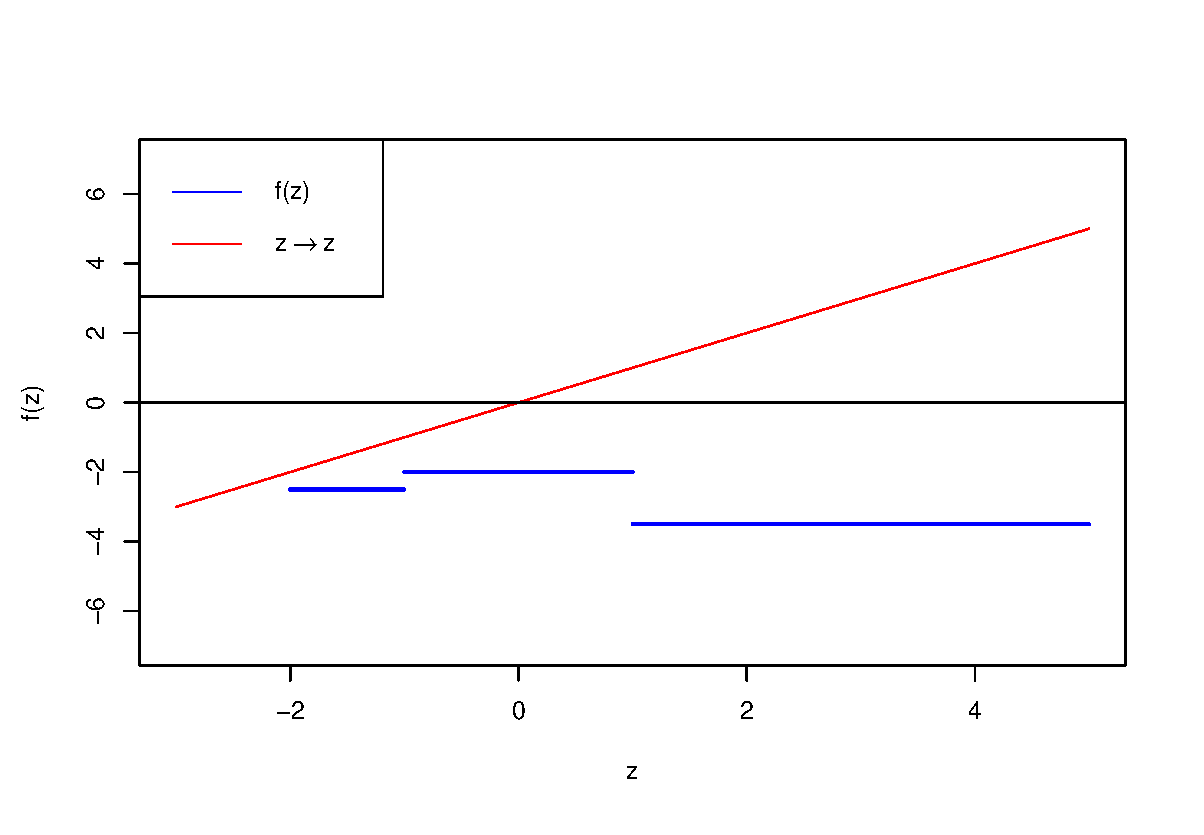
\includegraphics[scale=.5]{Clarke_Plot.eps}
\end{centering}
\end{frame}
\begin{frame}{Existence Counter-Example}
\begin{centering}
\includegraphics[scale=.5]{Clarke_Plot2.eps}
\end{centering}
\end{frame}

\begin{frame}{One Factor Model with Long Only Constraints (cont.)}
Reformulated Clarke Map.  First, assume without loss of generality $\be^\T \gb>0$.  Define $\psi: \bbr_+  \mapsto \bbr$:
\begin{equation}\label{psieq}
\psi(z) = \frac{\sum_{\{i:z\gb_i<1\}} \gb_i/\gd_i^2}{1/\gs^2+ \sum_{ \{i:z\gb_i<1\} } \gb_i^2/\gd_i^2}
\end{equation}
\begin{itemize}
\item This is the reciprocal of $\psi_C$ with a slightly different summand condition.
\item This is the same as the multidimensional $\psi(z) = \bA_z^{-1}b_z$ system introduced earlier, but with $q=1$.
\item We wish to find $\theta$ such that $\psi(\theta) = \theta$.  
\item$\psi(\cdot)$ is still a discontinuous step function; difficult to work with.
\end{itemize}
\end{frame}


\begin{frame}{One Factor Model with Long Only Constraints (cont.)}
\begin{lemma} Assume $\psi(0)>0$ (equiv. $\be^\T \gb>0$).  Define the function $\phi: \bbr_+ \mapsto \bbr$:
\begin{equation}\label{phi}
\phi(z) = -\gs^2\paren{ \sum_{\{i:z\gb_i<1\}} \frac{\gb_i}{\gd_i^2}\paren{z \gb_i-1}}.
\end{equation}
A fixed point $\phi(\theta) = \theta$ exists if and only if a fixed point of $\psi(\theta) = \theta$ exists; furthermore, the solutions have the same value.
\end{lemma}
Note that is is also the same as the $\varphi(z)=\bV \bB^\T \Gd^{-1}(\rme-\bB z)_+$ function for $q=1$.
\end{frame}

\begin{frame}{One Factor Model with Long Only Constraints (cont.)}
\begin{lemma}
For $\phi:\bbr_+ \mapsto \bbr$ as defined in Equation \req{phi}, we have the following:
\begin{enumerate}
\item $\phi(z)$ is continuous
\item $\phi(0)>0$
\item $\phi$ is differentiable a.e. and $\phi'(z)<0$ for all $z>0$
\item $\phi(z)$ has a positive root.
\end{enumerate}
\end{lemma}
\end{frame}




\begin{frame}{One Factor Model with Long Only Constraints (cont.)}
\begin{centering}
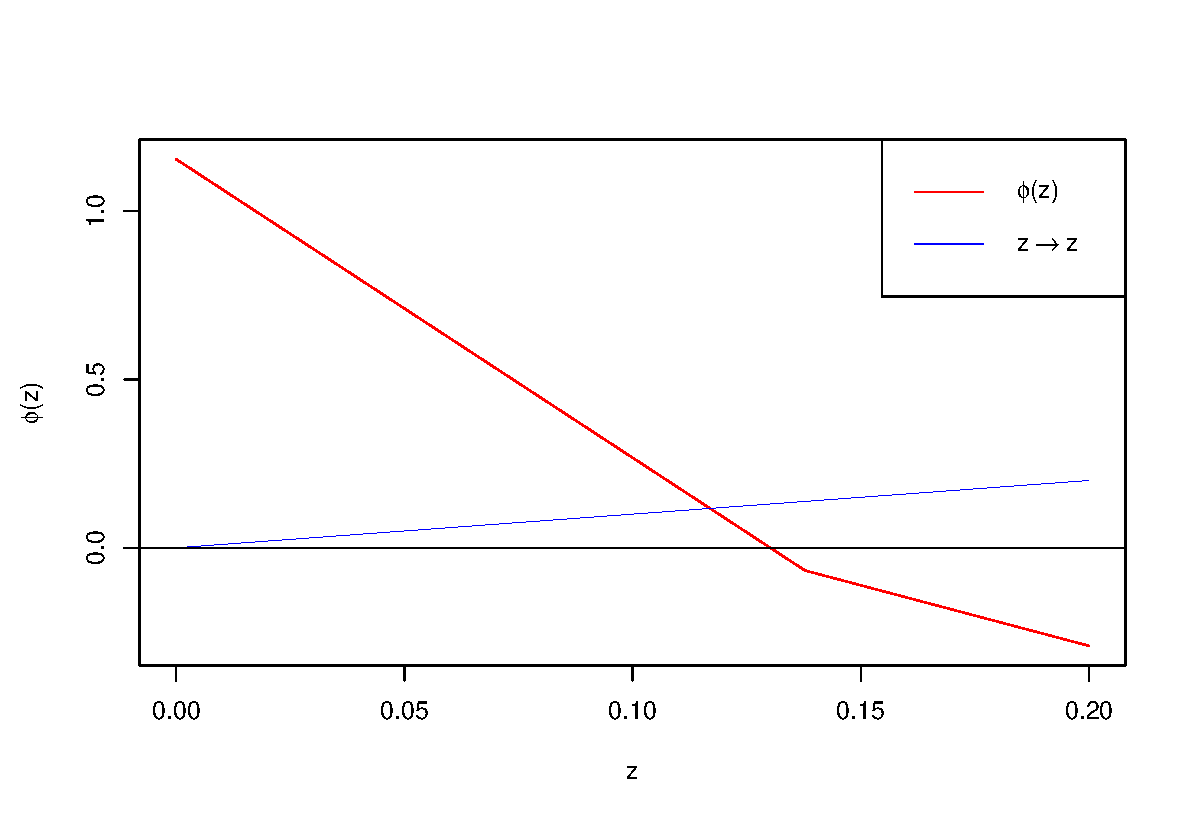
\includegraphics[scale=.5]{FP.eps}
\end{centering}
\end{frame}



\begin{frame}{One Factor Model with Long Only Constraints (cont.)}
\begin{theorem}
There exists a unique nonzero $\theta$ that solves $\phi(\theta)=\theta$
\end{theorem}
This solution is equivalent to the solution to Equation \req{psieq}.
\begin{proof}
This is a straightforward consequence of the Brouwer Fixed-Point Theorem, as  $\phi(\cdot)$ is continuous, $\phi(0)>0$ and for some $z>0$, $\phi(z)=0$.
\end{proof}
\end{frame}

\begin{frame}{Algorithm for One-Factor Model}
Goal: Compute the fixed-point in Equation \req{psieq} under the assumption that $\be^\T \gb/\gd^2 >0$ and $\theta>0$.\\
\textit{Note:} For $\theta$ large enough, $\psi(\theta)$ decreasing and the condition $\theta \gb_i<1$ ensures that every negative $\gb_i$ will be included in the summation.
\begin{itemize}
\item Order $\gb$ vector in increasing order.
\item Starting from $k=p$, compute 
\begin{equation}
\psi_k = \frac{\sum_{i=1}^k\gb_i/\gd_i^2}{1/\gs^2 \sum_{i=1}^k \gb_i^2/\gd_i^2}
\end{equation}
\item If $\psi_k \gb_k < 1$, stop, otherwise repeat for $k=k-1$.
\end{itemize}
\end{frame}


\section{Case Study}

\begin{frame}{Case Study: Sensitivity with Respect to Factor Variance}
\begin{itemize}
\item We now have semi-explicit formulae for the solutions of Long-Only Markowitz Portfolios which allow us to conduct a sensitivity analyses.
\item We want to understand the sensitivity $w_i$ (and thus $x_i$) with respect to factor variance, $\gs^2$.
\item \bambootext{With our formulae, we do not need to re-solve the quadratic program for every value we wish to check}
\end{itemize}
\end{frame}

\begin{frame}{Case Study: Sensitivity with Respect to Factor Variance}
For a fixed $\theta$, we can examine the following partial derivatives:
\begin{equation}
\diff {\gs^2} w_i  = -\frac{\gb_i}{\gd_i^2}\frac{\partial \theta}{\partial \gs^2}
\end{equation}
\begin{equation}
\diff {\gs^2} \theta  = \frac{(\phi(\theta)/\gs^2)}{1 + \gs^2 \sum_{\{i:\theta \gb_i <1 \}} \gb_i^2/\gd_i^2}
\end{equation}
\begin{equation}
\diff {\gs^2} w_i  = \frac{\gb_i \sum_{\{k: \theta \gb_k<1\}} (\gb_k/\gd_k^2)(\theta \gb_k-1)}{\gd_i^2 + \gd_i^2 \gs^2 \sum_{\{k:\theta \gb_k <1 \}} \gb_k^2/\gd_k^2}
\end{equation}
These are ugly formulae...
\end{frame}

\begin{frame}{Derivative of $w_i$ with Respect to $\gs^2$}
\begin{centering}
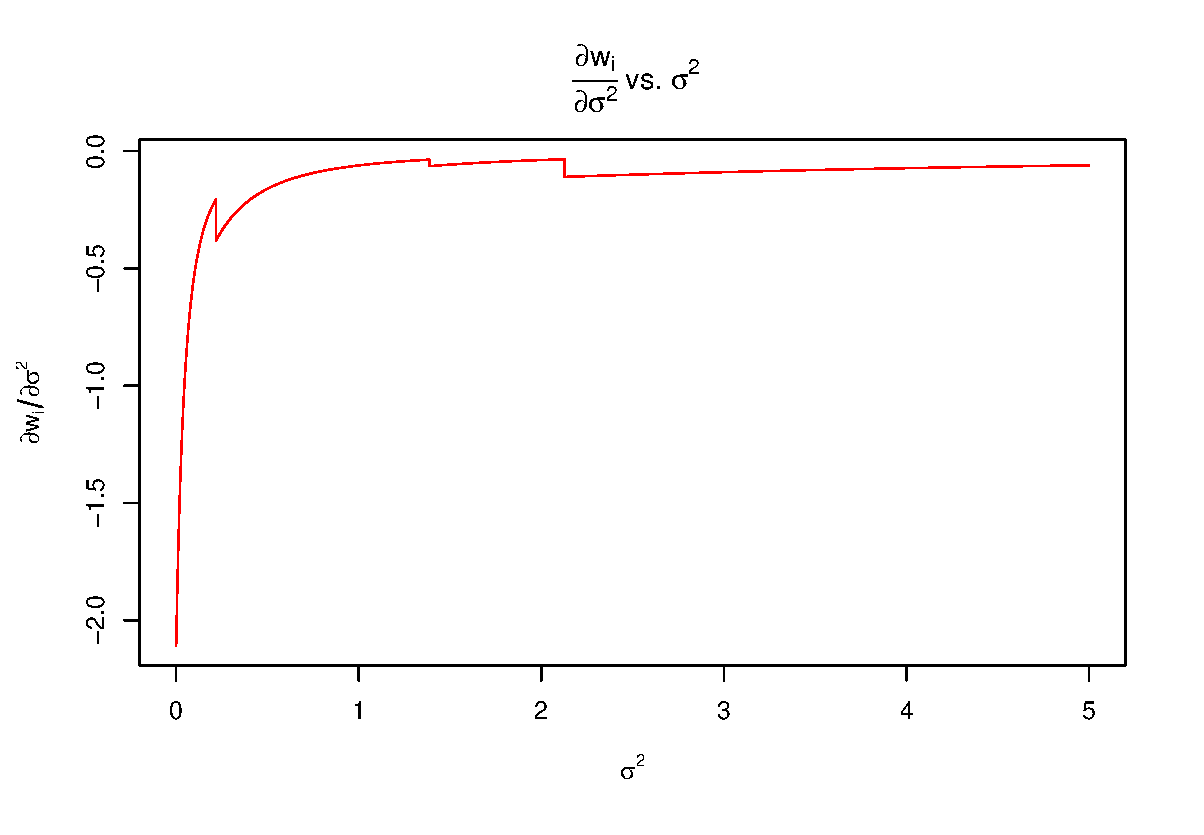
\includegraphics[scale=.5]{sigma_deriva.eps}
\end{centering}
$p=5$, $\gb \sim \ncal_5(1,1)$, $\gd_i^2\sim \mrm{lognorm}(0,1)$.
\end{frame}


\begin{frame}{Derivative of $w_i$ with Respect to $\gs^2$}
\begin{centering}
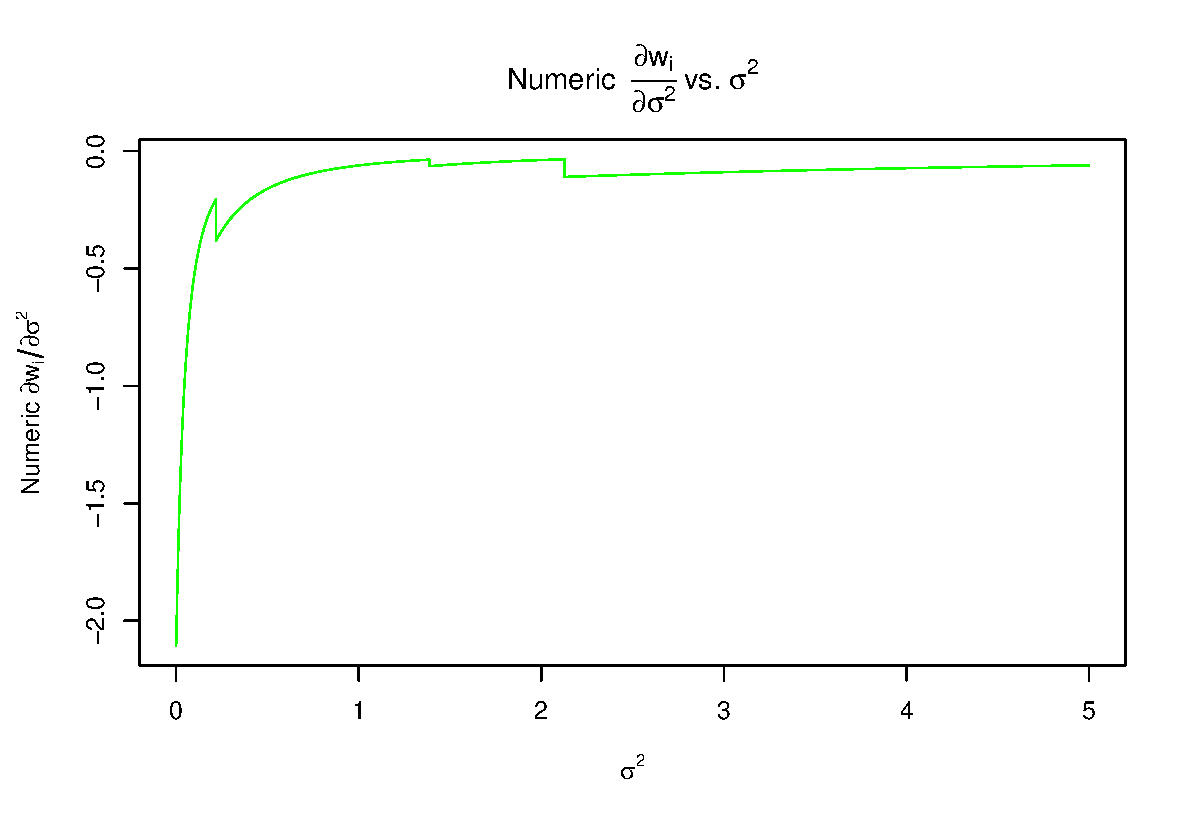
\includegraphics[scale=.5]{sigma_deriva_numeric.eps}
\end{centering}
$p=5$, $\gb \sim \ncal_5(1,1)$, $\gd_i^2\sim \mrm{lognorm}(0,1)$. \\ 
\footnotesize{Numeric Derivative is of $\theta$, computed over many values of $\gs^2$.}
\end{frame}

\begin{frame}{Comments}
\begin{itemize}
\item Numeric derivative computed by differencing solutions of $\theta$ rather than re-solving the quadratic program.
\item Numeric derivative and actual formula are very close
\item Furthermore, these can be very computationally difficult to estimate even in the $1$-Factor case without Fixed-Point formulation
\end{itemize}

\end{frame}

\section{Future Work}
\begin{frame}
\begin{itemize}
\item Include risk tolerance, and map these results to the entire efficient frontier
\item Generalize long-only constraints to arbitrary weight constraints
\item Study the implications of these weights for statistical estimation of covariance matrices
\end{itemize}
\end{frame}


\begin{frame}[allowframebreaks]{References}
\bibliography{siambib}
\bibliographystyle{jmr}

\end{frame}

\end{document}

